\documentclass[handout, 11pt]{beamer}
\mode
<presentation>{\usetheme{Madrid}}
\institute[UF]{\inst{1}
University of Florida\\
Department of Finance, Insurance, and Real Estate}
\usepackage{booktabs}
\usepackage{adjustbox}
\usepackage{tikz}
\definecolor{darkgreen}{RGB}{31,156,17}
\usepackage{minted}
\usepackage{xcolor}
\setbeamertemplate{headline}{\begin{beamercolorbox}[ht=2.25ex, dp=3.75ex]{section in head/foot}
\insertnavigation{\paperwidth}
\end{beamercolorbox}}
\AtBeginSection{\begin{frame}
\frametitle{Table of Contents}
\tableofcontents[currentsection]
\end{frame}}
\begin{document}
\title[Visualization]{Understanding Complex Results}
\subtitle{An Introduction to Visualization and \texttt{pandas}}
\author[DeRobertis]{Nick DeRobertis\inst{1}}
\date{\today}
\begin{frame}
\titlepage
\label{title-frame}
\end{frame}
\begin{section}[Intro]{Visualization Introduction}
\begin{frame}
\frametitle{Why Visualize?}
\begin{itemize}
\item So far we've had one main output from our model, number of years
\vfill
\item Salaries and wealth over time have also been outputs, but we haven't had a good way of understanding that output. It's a bunch of numbers.
\vfill
\item This is where visualization comes in. We have some complex result, and want to make it easily interpretable.
\end{itemize}
\end{frame}
\begin{frame}
\frametitle{What we Have so Far}
\begin{center}
\begin{tabular}{lcc}
\multicolumn{3}{c}{\textbf{Retirement Info}}\\
\cmidrule(lr){1-3}
Time & Salaries & Wealths\\
  1 &   61,200 &   31,050 \\
  2 &   62,424 &   48,208 \\
  3 &   63,672 &   66,537 \\
  4 &   64,946 &   86,100 \\
  5 &   76,182 &  109,451 \\
  6 &   77,705 &  134,350 \\
  7 &   79,259 &  160,882 \\
  8 &   80,844 &  189,137 \\
  9 &   82,461 &  219,209 \\
 10 &   96,727 &  254,352 \\
 11 &   98,662 &  291,735 \\
 12 &  100,635 &  331,480 \\

\end{tabular}
\end{center}
\end{frame}
\begin{frame}
\frametitle{Visualization in Excel}
\begin{center}
\begin{adjustbox}{width=0.9\textwidth, height=0.8\textheight, keepaspectratio}
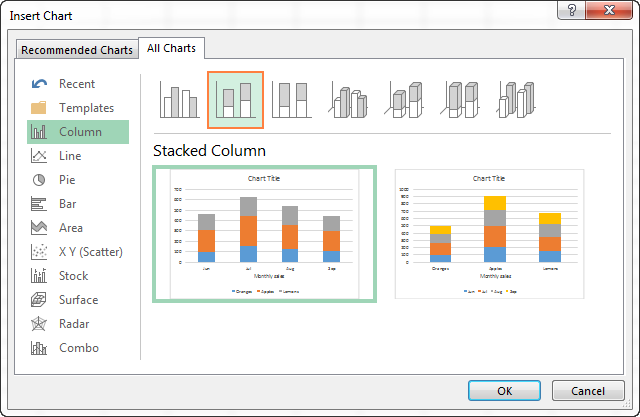
\includegraphics[width=1.0\textwidth]{Sources/excel-insert-chart.png}
\end{adjustbox}
\end{center}
\end{frame}
\begin{frame}
\frametitle{An Overwhelming Number of Options in Python}
\begin{center}
\begin{adjustbox}{width=0.9\textwidth, height=0.8\textheight, keepaspectratio}
\begin{tikzpicture}
\node [anchor=south west] (c76dabc2-1964-4a10-b72a-88fafa6f2138)  {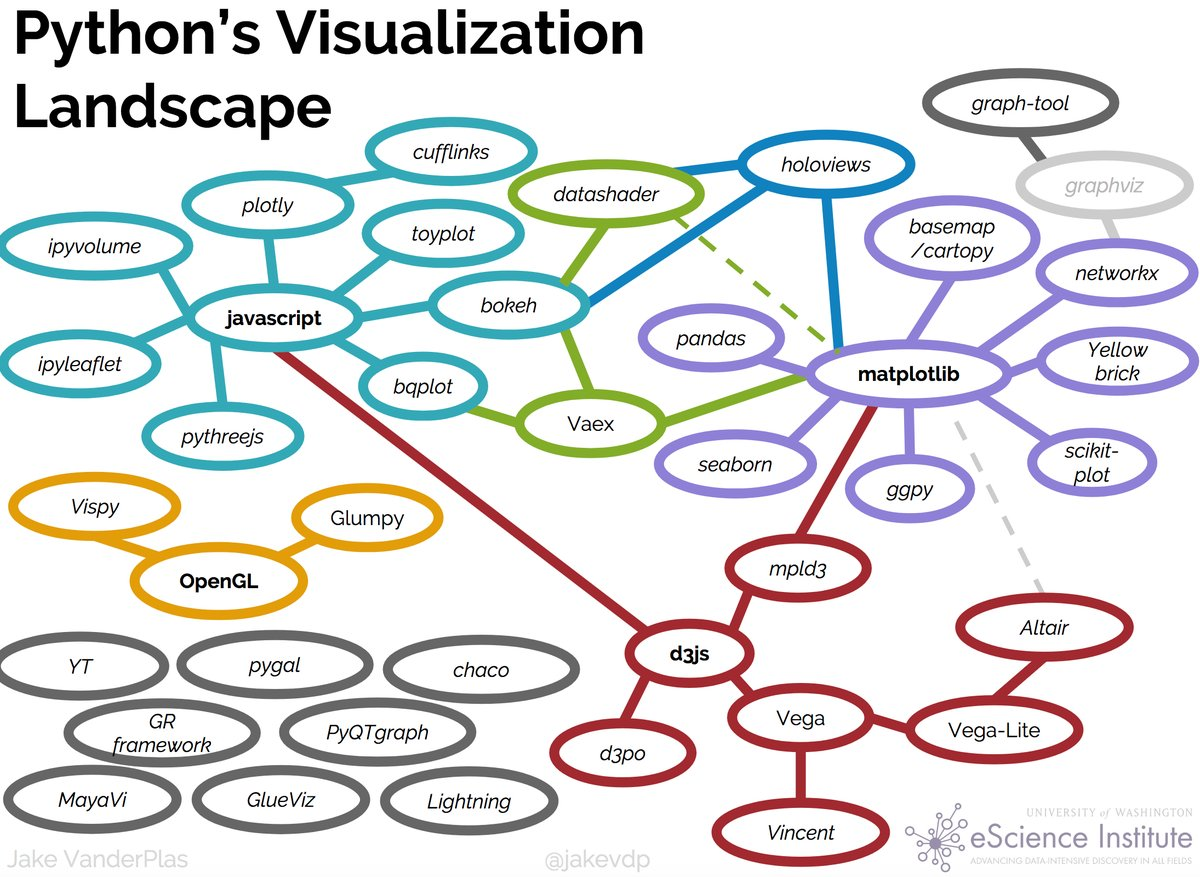
\includegraphics[width=1.0\textwidth]{Sources/python-visualization-landscape.jpg}};
\begin{scope}[x={(c76dabc2-1964-4a10-b72a-88fafa6f2138.south east)}, y={(c76dabc2-1964-4a10-b72a-88fafa6f2138.north west)}]
\path [draw, red] (0.52, 0.52) rectangle (0.85, 0.67);
\end{scope}
\end{tikzpicture}
\end{adjustbox}
\end{center}
\end{frame}
\begin{frame}
\frametitle{Explaining Python Visualization in This Class}
\begin{itemize}
\item Ultimately, we will be creating graphs using
\texttt{matplotlib}
but we won't use it directly.
\vfill
\item Instead, we will use
\texttt{pandas}
\vfill
\item \texttt{pandas}
is actually creating its graphs using
\texttt{matplotlib}
for us, but it is simpler to use.
\end{itemize}
\end{frame}
\begin{frame}
\frametitle{Visualization in Excel}
{
\setbeamercolor{block title}{bg=darkgreen}
\begin{block}{Adding Graphs to the Dynamic Salary Retirement Excel Model}
\begin{itemize}
\item I will now go back to the "Dynamic Salary Retirement Model.xlsx" Excel model to add visualization. If you do not have it already, it is in Examples > Intro > Excel. 
\item I have also uploaded the completed workbook from this exercise in Examples > Visualization > Excel > Dynamic Salary Retirement Model Visualized.xlsx
\item Follow along as I go through the example.
\end{itemize}
\end{block}
}
\end{frame}
\end{section}
\begin{section}[Pandas]{Tables with Pandas DataFrames}
\begin{frame}
\frametitle{Some Setup Before we can Visualize in Python}
\begin{itemize}
\item \texttt{pandas}
does
\textbf{a lot}
more than just graphing. We will use it throughout the rest of the class.
\vfill
\item Previously we've worked with lists, numbers, strings, and even our custom types (our model dataclasses)
\vfill
\item \texttt{pandas}
provides the
\texttt{DataFrame}
as a new type that we can use.
\vfill
\item Before we can get to graphing, we must learn how to use the \texttt{DataFrame}.
\end{itemize}
\end{frame}
\begin{frame}
\frametitle{What is a \texttt{DataFrame}?}
A
\texttt{DataFrame}
is essentially a table. It has rows and columns, just like in Excel.
\vfill
\begin{block}{Some Features of the \texttt{DataFrame}}
\begin{itemize}
\item Add or remove columns or rows
\item Group by and aggregate
\item Load in and output data from/to Excel and many other formats
\item Merge and join data sets
\item Reshape and pivot data
\item Time-series functionality
\item Slice and query your data
\item Handle duplicates and missing data
\end{itemize}
\end{block}
\end{frame}
\begin{frame}[fragile]
\frametitle{A Basic \texttt{DataFrame} Example}
\begin{minted}{python}

>>> import pandas as pd
>>> df = pd.DataFrame()
>>> df['Sales'] = [1052, 212, 346]
>>> df['Category'] = ['Aprons', 'Apples', 'Bowties']
df

\end{minted}
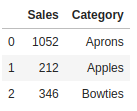
\includegraphics[width=0.3\textwidth]{Sources/df-basic-example.png}
\end{frame}
\begin{frame}
\frametitle{Introduction to Pandas}
{
\setbeamercolor{block title}{bg=darkgreen}
\begin{block}{Creating and Using Pandas DataFrames}
\begin{itemize}
\item I will now go through the notebook in Examples > Visualization > Python > Intro to Pandas and Table Visualization.ipynb
\item Follow along as I go through the example.
\item We will complete everything up until DataFrame Styling
\end{itemize}
\end{block}
}
\end{frame}
\begin{frame}
\frametitle{Intro Pandas Lab}
{
\setbeamercolor{block title}{bg=violet}
\begin{block}{Getting Started with Pandas}
\begin{enumerate}
\item Work off of the Jupyter notebook Pandas and Visualization Labs.ipynb
\item Complete the lab exercises in the first section entitled "Pandas"
\end{enumerate}
\vfill
\begin{tabular*}{\textwidth}{@{\extracolsep{\fill}}ccc}
\toprule
\hfill & Resources: Slide \textcolor{blue}{\underline{\ref{labs:intro-pandas-lab-1-resources}}} & \hfill\\

\end{tabular*}
\end{block}
}
\label{labs:intro-pandas-lab-1}
\end{frame}
\begin{frame}
\frametitle{Styling Pandas DataFrames}
\begin{itemize}
\item It is possible to add styling to our displayed tabular data by styling the
\texttt{DataFrame}
\vfill
\item The styling is very flexible and essentially allows you to do anything
\vfill
\item Out of the box, it is easy to change colors, size, and positioning of text, add a caption, do conditional formatting, and draw a bar graph over the cells.
\end{itemize}
\end{frame}
\begin{frame}
\frametitle{Introduction to Pandas}
{
\setbeamercolor{block title}{bg=darkgreen}
\begin{block}{Creating and Using Pandas DataFrames}
\begin{itemize}
\item I will now go through the next section in Examples > Visualization > Python > Intro to Pandas and Table Visualization.ipynb
\item Follow along as I go through the example.
\item This time we are covering the remainder of the notebook starting from "DataFrame Styling"
\end{itemize}
\end{block}
}
\end{frame}
\begin{frame}
\frametitle{Pandas Styling Lab}
{
\setbeamercolor{block title}{bg=violet}
\begin{block}{Styling Pandas DataFrames}
\begin{enumerate}
\item Keep working with the same lab Jupyter Notebook
\item Complete the lab exercises in the second section entitled "Pandas Styling"
\end{enumerate}
\vfill
\begin{tabular*}{\textwidth}{@{\extracolsep{\fill}}ccc}
\toprule
\hfill & Resources: Slide \textcolor{blue}{\underline{\ref{labs:pandas-styling-lab-1-resources}}} & \hfill\\

\end{tabular*}
\end{block}
}
\label{labs:pandas-styling-lab-1}
\end{frame}
\end{section}
\begin{section}[Graphs]{Graphing using Pandas}
\begin{frame}[fragile]
\frametitle{A Minimal Plotting Example}
\begin{block}{Line Graphs using \texttt{pandas}}
\begin{minted}{python}

>>> %matplotlib inline
>>> ret_df.plot.line(x='Time', y='Salaries')

\end{minted}
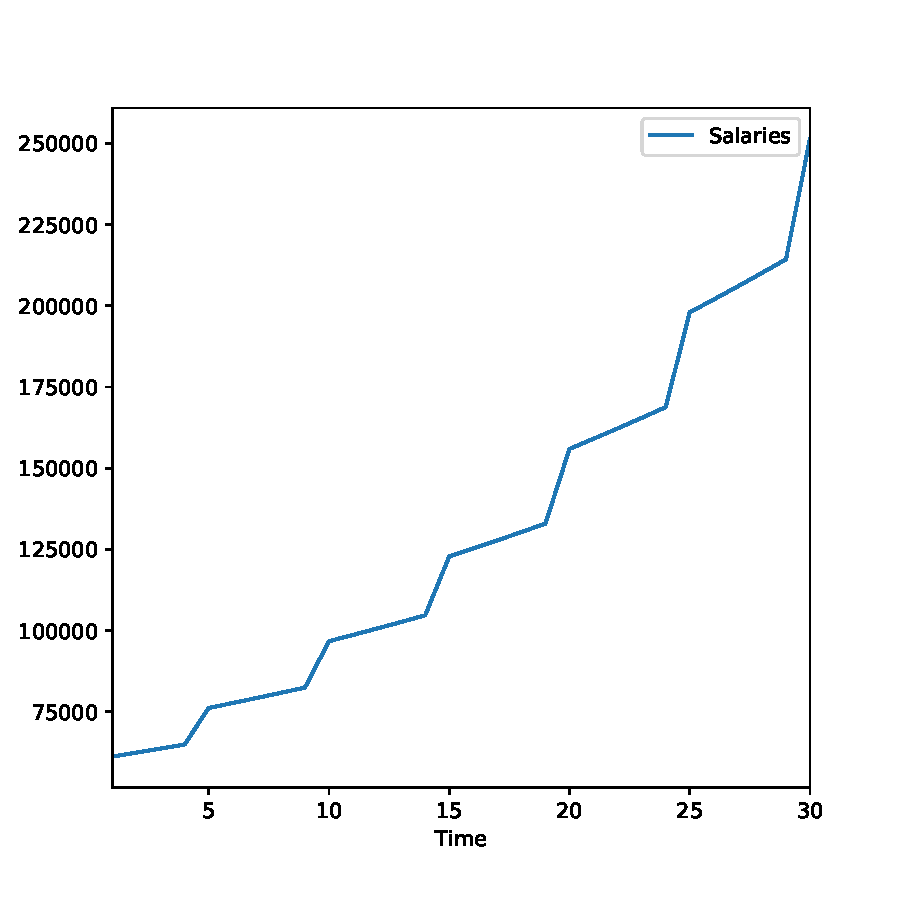
\includegraphics[width=0.5\textwidth]{Sources/python-salaries-line-graph.pdf}
\end{block}
\end{frame}
\begin{frame}
\frametitle{Basic Graph Types: Line Graphs}
\begin{adjustbox}{width=0.425\textwidth, height=0.8\textheight, keepaspectratio}
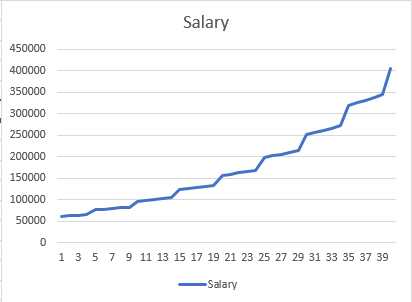
\includegraphics[width=1.0\textwidth]{Sources/excel-salaries-line-graph.png}
\end{adjustbox}
\hfill
\begin{adjustbox}{width=0.425\textwidth, height=0.8\textheight, keepaspectratio}
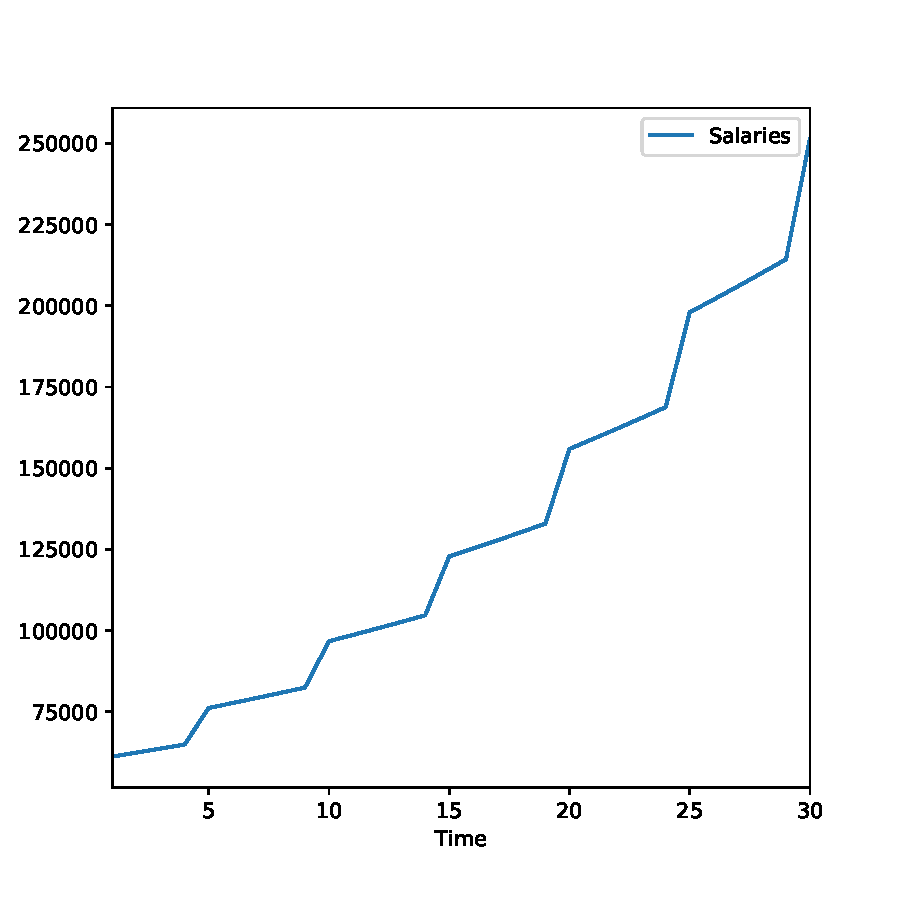
\includegraphics[width=1.0\textwidth]{Sources/python-salaries-line-graph.pdf}
\end{adjustbox}
\end{frame}
\begin{frame}
\frametitle{Basic Graph Types: Bar Graphs}
\begin{adjustbox}{width=0.425\textwidth, height=0.8\textheight, keepaspectratio}
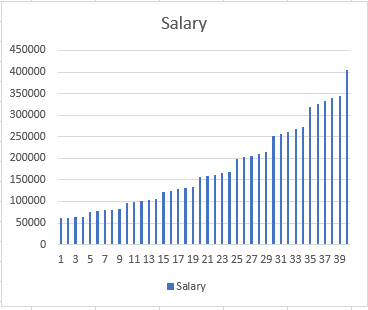
\includegraphics[width=1.0\textwidth]{Sources/excel-salaries-bar-graph.png}
\end{adjustbox}
\hfill
\begin{adjustbox}{width=0.425\textwidth, height=0.8\textheight, keepaspectratio}
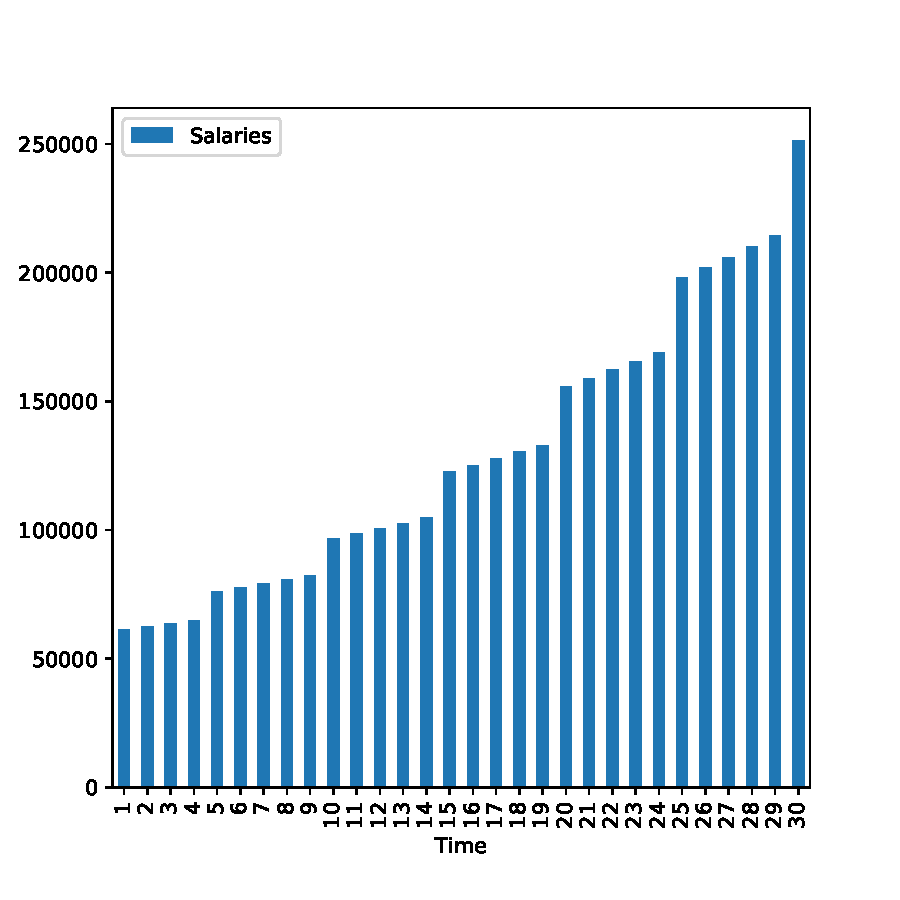
\includegraphics[width=1.0\textwidth]{Sources/python-salaries-bar-graph.pdf}
\end{adjustbox}
\end{frame}
\begin{frame}
\frametitle{Basic Graph Types: Box and Whisker Plots}
\begin{adjustbox}{width=0.425\textwidth, height=0.8\textheight, keepaspectratio}
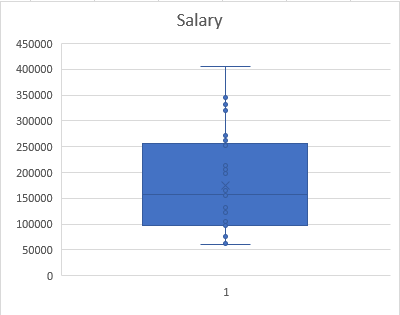
\includegraphics[width=1.0\textwidth]{Sources/excel-salaries-box-whisker-plot.png}
\end{adjustbox}
\hfill
\begin{adjustbox}{width=0.425\textwidth, height=0.8\textheight, keepaspectratio}
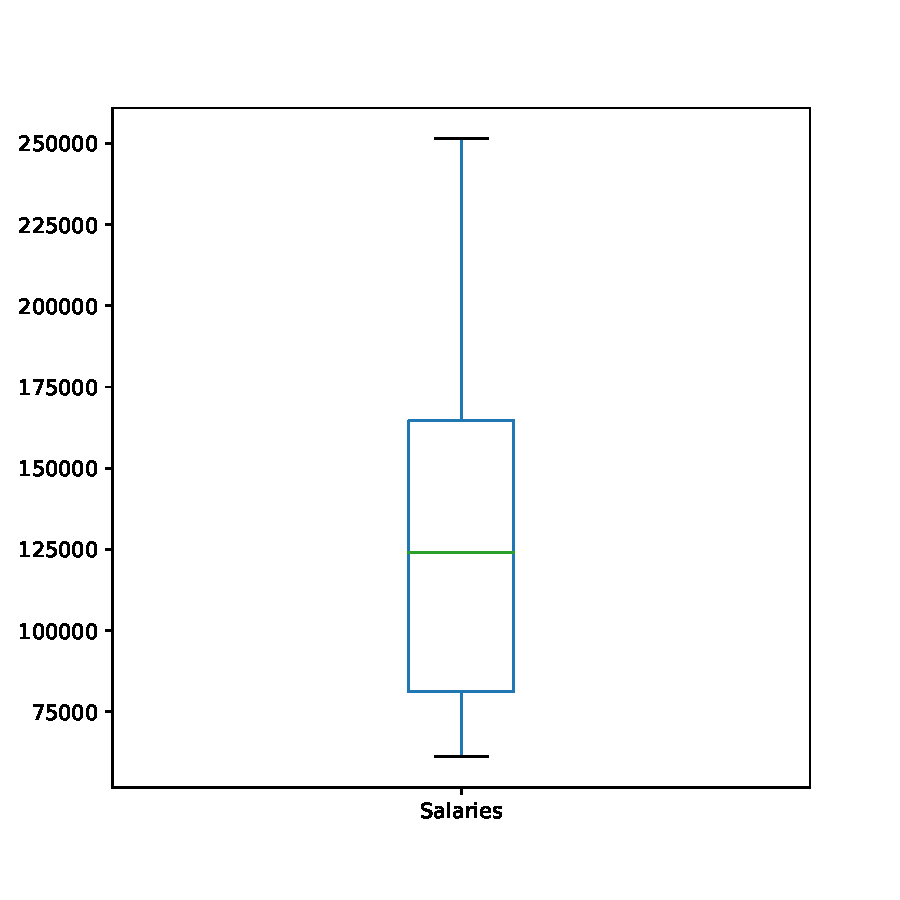
\includegraphics[width=1.0\textwidth]{Sources/python-salaries-box-graph.pdf}
\end{adjustbox}
\end{frame}
\begin{frame}
\frametitle{Introduction to Graphing}
{
\setbeamercolor{block title}{bg=darkgreen}
\begin{block}{Graphing Using Pandas}
\begin{itemize}
\item I will now go through Examples > Visualization > Python > Intro to Graphics.ipynb
\item Follow along as I go through the entire example notebook.
\end{itemize}
\end{block}
}
\end{frame}
\begin{frame}
\frametitle{Intro Visualization Lab}
{
\setbeamercolor{block title}{bg=violet}
\begin{block}{Introduction to Graphing with Pandas}
\begin{enumerate}
\item Keep working with the same lab Jupyter Notebook
\item Complete the lab exercises in the final section entitled "Graphics"
\end{enumerate}
\vfill
\begin{tabular*}{\textwidth}{@{\extracolsep{\fill}}ccc}
\toprule
\hfill & Resources: Slide \textcolor{blue}{\underline{\ref{labs:intro-visualization-lab-1-resources}}} & \hfill\\

\end{tabular*}
\end{block}
}
\label{labs:intro-visualization-lab-1}
\end{frame}
\end{section}
\appendix
\newcounter{finalframe}
\setcounter{finalframe}{\value{framenumber}}
\begin{frame}
\frametitle{Lecture Resources}
{
\setbeamercolor{block title}{bg=teal}
\begin{block}{Lecture Resources}
\begin{enumerate}
\item \textcolor{blue}{\underline{\href{https://nickderobertis.github.io/fin-model-course/\_static/generated/pdfs/S6 Understanding Complex Results.pdf}{Slides - Understanding Complex Results}}}
\item \textcolor{blue}{\underline{\href{https://nickderobertis.github.io/fin-model-course/\_static/generated/pdfs/LN6 Understanding Complex Results.pdf}{Lecture Notes - Understanding Complex Results}}}
\item \textcolor{blue}{\underline{\href{https://nickderobertis.github.io/fin-model-course/\_static/Examples/Visualization/Excel/Dynamic Salary Retirement Model Visualized.xlsx}{Dynamic Salary Retirement Model Visualized}}}
\item \textcolor{blue}{\underline{\href{https://nickderobertis.github.io/fin-model-course/\_static/Examples/Visualization/Python/Intro to Pandas and Table Visualization.ipynb}{Intro to Pandas and Table Visualization}}}
\item \textcolor{blue}{\underline{\href{https://nickderobertis.github.io/fin-model-course/\_static/Materials for Lab Exercises/Visualization/Pandas and Visualization Labs.ipynb}{Pandas and Visualization Labs}}}
\item \textcolor{blue}{\underline{\href{https://nickderobertis.github.io/fin-model-course/\_static/Examples/Visualization/Python/Intro to Graphics.ipynb}{Intro to Graphics}}}
\item \textcolor{blue}{\underline{\href{https://nickderobertis.github.io/fin-model-course/\_static/Examples/Visualization/Python/Dynamic Salary Retirement Model Visualized.ipynb}{Dynamic Salary Retirement Model Visualized}}}
\end{enumerate}
\vfill
\end{block}
}
\label{frames:resources}
\end{frame}
\begin{frame}
\frametitle{Intro Pandas Lab Resources}
{
\setbeamercolor{block title}{bg=teal}
\begin{block}{Getting Started with Pandas Resources}
\begin{enumerate}
\item \textcolor{blue}{\underline{\href{https://nickderobertis.github.io/fin-model-course/\_static/Materials for Lab Exercises/Visualization/Pandas and Visualization Labs.ipynb}{Pandas and Visualization Labs}}}
\item \textcolor{blue}{\underline{\href{https://nickderobertis.github.io/fin-model-course/\_static/generated/pdfs/S6 Understanding Complex Results.pdf}{Slides - Understanding Complex Results}}}
\end{enumerate}
\vfill
\begin{tabular*}{\textwidth}{@{\extracolsep{\fill}}ccc}
\toprule
\hfill & Exercise: Slide \textcolor{blue}{\underline{\ref{labs:intro-pandas-lab-1}}} & \hfill\\

\end{tabular*}
\end{block}
}
\label{labs:intro-pandas-lab-1-resources}
\end{frame}
\begin{frame}
\frametitle{Pandas Styling Lab Resources}
{
\setbeamercolor{block title}{bg=teal}
\begin{block}{Styling Pandas DataFrames Resources}
\begin{enumerate}
\item \textcolor{blue}{\underline{\href{https://nickderobertis.github.io/fin-model-course/\_static/Materials for Lab Exercises/Visualization/Pandas and Visualization Labs.ipynb}{Pandas and Visualization Labs}}}
\item \textcolor{blue}{\underline{\href{https://nickderobertis.github.io/fin-model-course/\_static/generated/pdfs/S6 Understanding Complex Results.pdf}{Slides - Understanding Complex Results}}}
\end{enumerate}
\vfill
\begin{tabular*}{\textwidth}{@{\extracolsep{\fill}}ccc}
\toprule
\hfill & Exercise: Slide \textcolor{blue}{\underline{\ref{labs:pandas-styling-lab-1}}} & \hfill\\

\end{tabular*}
\end{block}
}
\label{labs:pandas-styling-lab-1-resources}
\end{frame}
\begin{frame}
\frametitle{Intro Visualization Lab Resources}
{
\setbeamercolor{block title}{bg=teal}
\begin{block}{Introduction to Graphing with Pandas Resources}
\begin{enumerate}
\item \textcolor{blue}{\underline{\href{https://nickderobertis.github.io/fin-model-course/\_static/Materials for Lab Exercises/Visualization/Pandas and Visualization Labs.ipynb}{Pandas and Visualization Labs}}}
\item \textcolor{blue}{\underline{\href{https://nickderobertis.github.io/fin-model-course/\_static/generated/pdfs/S6 Understanding Complex Results.pdf}{Slides - Understanding Complex Results}}}
\end{enumerate}
\vfill
\begin{tabular*}{\textwidth}{@{\extracolsep{\fill}}ccc}
\toprule
\hfill & Exercise: Slide \textcolor{blue}{\underline{\ref{labs:intro-visualization-lab-1}}} & \hfill\\

\end{tabular*}
\end{block}
}
\label{labs:intro-visualization-lab-1-resources}
\end{frame}
\setcounter{framenumber}{\value{finalframe}}
\end{document}